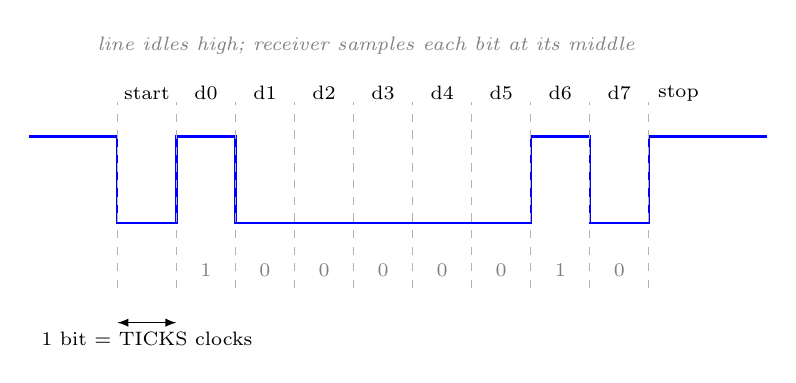
\begin{tikzpicture}[x=0.75cm,y=1.1cm, >=latex]
% frame for 'A' = 0x41, LSB first: idle 1 | start 0 | 1,0,0,0,0,0,1,0 | stop 1
\draw[thick, blue] (-0.5,1) -- (1,1) -- (1,0) -- (2,0) -- (2,1) -- (3,1)
  -- (3,0) -- (8,0) -- (8,1) -- (9,1) -- (9,0) -- (10,0) -- (10,1) -- (12,1);
\foreach \x/\n in {1.5/start,2.5/{d0},3.5/{d1},4.5/{d2},5.5/{d3},6.5/{d4},7.5/{d5},8.5/{d6},9.5/{d7},10.5/stop}
  \node[font=\scriptsize] at (\x,1.5) {\n};
\foreach \x/\v in {2.5/1,3.5/0,4.5/0,5.5/0,6.5/0,7.5/0,8.5/1,9.5/0}
  \node[font=\scriptsize, text=gray] at (\x,-0.55) {\v};
\foreach \x in {1,...,10} \draw[gray!60, dashed] (\x,-0.75) -- (\x,1.4);
\draw[<->] (1,-1.15) -- (2,-1.15) node[midway, below, font=\scriptsize] {1 bit = TICKS clocks};
\node[font=\scriptsize\itshape, anchor=west, gray] at (0.5,2.05)
  {line idles high; receiver samples each bit at its middle};
\end{tikzpicture}
